\chapter{Teoretická část}
%TODO write something nice

%%%%%%%%%%%%%%%%%%%%%%%%%%%%%%%%%%%%%%%%%%%%%%%%%
\section{Grafové databáze}

Grafy jsou velice přirozeným způsobem reprezentaci dat, zvláště v době, kdy většina dat je vytvářena uživateli v nestrukturované formě. Grafy pomocí uzlů a hran popisují objekty a vztahy mezi nimi s elegancí a přirozeností, jaké mohou jiné reprezentace dat těžko dosáhnout. Grafy usnadňují proces objevování informací v datech a přitom nevynucují náročné datové modelování skutečnosti do složitých datových struktur. Díky tomu, že grafy umožňují jednoduché prohladávání objektů, které mezi sebou mají vztahy (uzlů propojených hranami), jsou operace tohoto typu nad grafy relativně\footnote{Například vůči \nom{RDBMS}{relačním databázím} - čas nutný pro průchod přes několik hran je výrazně nižší než čas nutný ke spojení několika tabulek.} levné. 

\nom{GDB}{Grafové databáze} umožňují data reprezentovaná grafem ukládat a procházet tak, aby byly tyto přirozené výhody grafů zachovány a zároveň byly zajištěny alespoň některé vlastnosti \nom{RDBMS}{relačních databázových systémů}. 
% todo case studies https://neo4j.com/resources/top-use-cases-graph-databases-white-paper/

\subsection{Grafy}
% Matematická definice
Před popisem vlastních \nom{GDB}{grafových databází} blíže popíšeme grafy jako takové a jejich typy. Nejdříve uvedeme základní matematický rámec teorie grafů, se kterým budeme dále pracovat. 

Graf G je trojice (V, E, $\epsilon$), kde V je množina vrcholů\footnote{nebo také uzlů} a E množina hran. $\epsilon$ je přiřazení, které každé hraně přiřazuje: 
\begin{itemize} 
	\item{} množinu dvou vrcholů (koncové vrcholy) pro \textit{neorientovaný graf}
	\item{} uspořádanou dvojici vrzcholů (počáteční a koncový vrchol) pro \textit{orientovaný graf}
\end{itemize}

% Multigrafy / prosté grafy
Pokud graf neobsahuje paralelní hrany\footnote{nebo také multihrany}, tedy hrany, které mají stejné počáteční a koncové vrcholy (orientovaný graf), respektive stejné koncové vrcholy (neorientovaný graf), je označován jako \textit{prostý graf}. Naopak pokud graf paralelní hrany obsahuje, je označován jako \textit{multigraf}.\cite{Demlova17}

% Labeled grafy
Grafy z pohledu informačních technologií matematickou definici grafu dále rozšiřují. Umožňují definovat typy hran a uzlů, čímž vzniká \textit{ohodnocený graf}\footnote{Ohodnocený graf bývá také často označován jako labeled graf. Jeho opakem, tedy "neohodnoceným" grafem je jednovztahový nebo také homogenní graf.} Například ohodnocený graf na obrázku \ref{fig:labeled_graf} obsahuje dva typy uzlů (:OSOBA a :ČLÁNEK) a dva typy hran (:ZNÁ a :ČETL).

\begin{figure}
\begin{center}
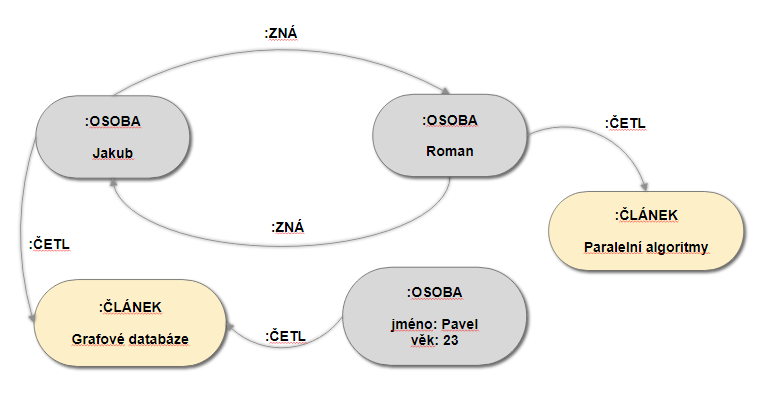
\includegraphics[width=14cm]{figures/labeled_graph}
\caption{Ohodnocený graf}
\label{fig:labeled_graf}
\end{center}
\end{figure}

% Property grafy
Ohodnocené grafy nám sice poskytují možnost rozlišit typy hran a uzlů, v mnoha situacích je ale žádoucí zachytit do grafu více informací. \textit{Atributové grafy} umožňují přiřadit hranám a uzlům libovolný počet atributů (dvojic klíč-hodnota), které obsahují informace o daném uzlu, respektive hraně. Příkladem může být věk osob, či datum vydání článku (viz obrázek \ref{fig:property_graf}). Většina grafových databází pracuje právě s atributovými grafy.\cite{Lal15}

\begin{figure}
\begin{center}
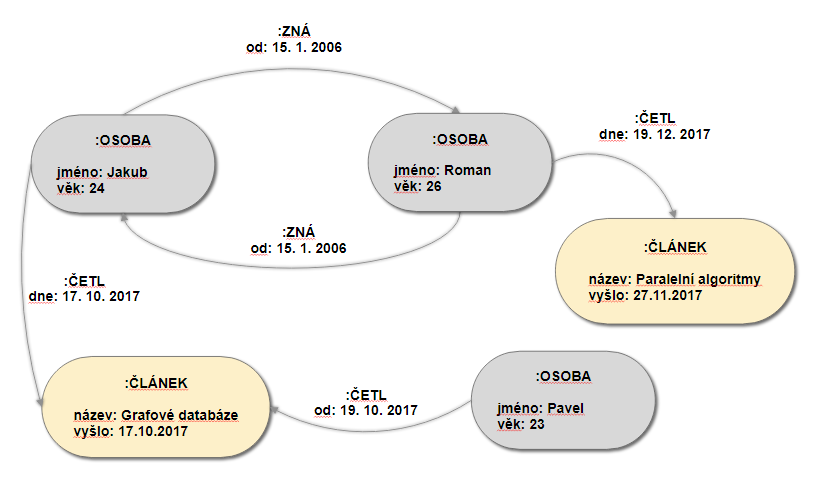
\includegraphics[width=14cm]{figures/property_graph}
\caption{Atributový graf}
\label{fig:property_graf}
\end{center}
\end{figure}

% Hypergrafy
Generalizací grafu je tzv. \textit{hypergraf}. Ten se proti grafu liší tím, že zatímco hrana grafu je množinou právě dvou vrcholů (či uspořádanou dvojicí v případě orientovaného grafu), hyperhrana (tedy hrana v hypergrafu) je mnoužinou jednoho a více vrcholů.\cite{Diestel00} Hypergrafy jsou používány k reprezentaci dat v mnoha oborech a některé GDB je přímo podporují (například HypergraphDB\footnote{http://hypergraphdb.org/}).


%TODO
\subsection{Perzistence}
%Přestože GDB jsou relativně novým pojmem ve světě informačních technologií (TODO cite vypuštění Neo4J), potřeba perzistence dat ve formě grafů byla i dříve. 

%TODO ukládání grafů
% RDBMS (NEO Reasons to use graph databases)
% Grafové struktury
% - adj matrix
% - adj list
% - inc matric
% - laplacean matrix
% - COMPRESSED ADJACENCY LISTS
% RDF
% - (haxtree)
% - (bitmap)

% TODO prostorová lokalita


%TODO
\subsection{Dotazování}
%todo možná samostatná sekce?

%typy dotazů 
% - podgraf
% - nadgrafb


%TODO
\subsection{Indexy}
% - mining based 
% - non-mining base 

%TODO
\subsection{Transakce}

%TODO
\subsection{Paralelizace}
%TODO Partitioning

%TODO 
\subsection{Databáze - příklady}


%%%%%%%%%%%%%%%%%%%%%%%%%%%%%%%%%%%%%%%%%%%%%%%%%
\section{Architektury a API} %todo maybe better heading
% https://cw.fel.cvut.cz/wiki/courses/a4m36aos/useful_materials

%todo RPC

%todo CORBA

%todo Java RMI

%todo mention HTTP 1.0 specification 1996

%todo mention XML specification 1996

%todo XML-RPC 
\subsection{XML-RPC}
V roce 1998 se objevil soubor pravidel, který popisuje jak využívat technilogie RPC, XML a HTTP k vzdálenému volání procedur přes internet - \nom{XML-RPC}{Remote Procedure Calling protokol používající XML pro komuniakci přes internet}.\cite{Winner99} XML poskytuje slovník pro popis RPC volání přenášená mezi počítači pomocí HTTP protokolu (ačkoliv je popsán také obecný přístup nezávislý na konkrétním protokolu). Uživatel pošle požadavek na server implementující protokol. Uživatelem je typicky software volající konkrétní proceduru vzdáleného systému. Volání může obasahovat více vstupních parametrů a očekává jedny výstupní hodnotu. Vstupní parametry mohou být vnořené do kolekcí jako jsou mapy a listy, mohou být tedy posílány rozsáhlé struktury. Proto je možné používat XML-RPC pro posílání objektů a struktur (jako vstupních i výsupních parametrů). Díky možnosti popsání předávaných informací pomocí XML umožňuje XML-RPC prakticky vytváření \nomExpl{API}{aplikačních rozhraní} a tím komunikaci dvou a více nehomogeních prostředí.\cite{Laurent01}  
% Because XML-RPC is layered on top of HTTP, it inherits the inefficiencies of HTTP. This
% does place some limitations on its use in large-scale, high-speed applications, but inefficiency
% isn't important in many places. Although there are definitely high-profile projects for which
% systems must scale to millions of transactions at a time, keeping response time to a minimum,
% there are also many projects to which systems need to send information or request
% processing far less often -- from once a second to once a week -- and for which response
% time isn't absolutely critical. For these cases, XML-RPC can simplify developers' lives
% tremendously. 

%todo SOAP, maybe UDDI and WSDL, maybe JAX-RPC
\subsection{SOAP}
Nástupcem XML-RPC se stal \nomExpl{SOAP}{Simple Object Access Protocol}. SOAP je postavený na podobných principech jako XML-RPC - používá XML jako formát zpráv a pro jejich přenos využívá protokolů aplikační vrstvy HTTP (standard), nebo SMTP. Cílem SOAPu je zajistit rozšířitelnost, neutralitu a nezávislost komunikace. Umožňuje komukaci procesů běžících na různých operačních systémech (pomocí XML) a volání webových služeb pomocí HTTP nezávisle na platformě a programovacím jazyku. 
Přestože specifikace SOAPu byla vytvořena už v roce 1998, byla zveřejněna až v roce 1999. Draft se nicméně nestal standardem \nomExpl{IETF}{Internet Engineering Task Force}\footnote{https://www.ietf.org/}.\cite{Box01} Až verze 1.2 se stala v roce 2007 doporučením \nomExpl{W3C}{World Wide Web Consortium}\footnote{https://www.w3.org/}.\cite{W3C07}
% https://en.wikipedia.org/wiki/SOAP
% https://www.w3.org/TR/2000/NOTE-SOAP-20000508/
% https://www.w3.org/TR/soap/

\nomExpl{WSDL}{Web Service Description Language} je formální strojově čitelný popis webové služby. Služba je popsána pomocí portů a koncových bodů


The WSDL describes services as collections of network endpoints, or ports. The WSDL specification provides an XML format for documents for this purpose. The abstract definitions of ports and messages are separated from their concrete use or instance, allowing the reuse of these definitions. A port is defined by associating a network address with a reusable binding, and a collection of ports defines a service. Messages are abstract descriptions of the data being exchanged, and port types are abstract collections of supported operations. The concrete protocol and data format specifications for a particular port type constitutes a reusable binding, where the operations and messages are then bound to a concrete network protocol and message format. In this way, WSDL describes the public interface to the Web service.
WSDL is often used in combination with SOAP and an XML Schema to provide Web services over the Internet. A client program connecting to a Web service can read the WSDL file to determine what operations are available on the server. Any special datatypes used are embedded in the WSDL file in the form of XML Schema. The client can then use SOAP to actually call one of the operations listed in the WSDL file using for example XML over HTTP.
The current version of the specification is 2.0; version 1.1 has not been endorsed by the W3C but version 2.0 is a W3C recommendation.[1] WSDL 1.2 was renamed WSDL 2.0 because of its substantial differences from WSDL 1.1. By accepting binding to all the HTTP request methods (not only GET and POST as in version 1.1), the WSDL 2.0 specification offers better support for RESTful web services, and is much simpler to implement.[2][3] However support for this specification is still poor in software development kits for Web Services which often offer tools only for WSDL 1.1.[needs update][citation needed] For example, the version 2.0 of the Business Process Execution Language (BPEL) only supports WSDL 1.1.


%todo REST
% http://roy.gbiv.com/talks/200709_fielding_rest.pdf
% fielding disertation

%todo HATEOS

%%%%%%%%%%%%%%%%%%%%%%%%%%%%%%%%%%%%%%%%%%%%%%%%%
\section{Data Layer}

\section{Data(base) Layer Abstraction}
Abstrakce datové vrstvy (a databází) je historicky hojně diskutovaným tématem, %TODO zdroj
střetává se zde několik zájmů. Nejčastější argumenty proti tomuto principu míří na 
ztrátu výkonost při zařazování abstraktních vrstev. Tato ztráta výkonu je potom často způsobena 
právě úrovní abstrakce, konkrétně neschopností vývojáře použít konstrukty specifické pro dané databázové systémy. 
Je ale důležité si uvědomit, že odstranění vendor lockingu není jediným a ani primárním cílem \nom{DLA}{Database Layer Abstraction}.
Důležitějším cílem je zjednodušení aplikační logiky a její očištění o konstrukty z databázového světa. 

%TODO úrovně abstrakce viz http://blog.gauffin.org/2013/01/data-layer-the-right-way/ + dohledat lepší zdroj

%TODO data access alternatives - pokud to není to samé, ten samý zdroj

%TODO Data layer patterns -ten samý zdroj + https://thinkinginobjects.com/2012/08/26/dont-use-dao-use-repository/ or https://medium.com/@krzychukosobudzki/repository-design-pattern-bc490b256006 
% and https://martinfowler.com/eaaCatalog/repository.html (!)

%==================================%
%              NOTES               %
%==================================%

% - domain and data mapping layer